
\section{Overlap between different categories}
\label{sec:overlap}

As has been discussed in Sect.~\ref{sec:analysis}, while the optimization of each
category is performed in an inclusive analysis, after having determine the order
of significance of the categories we turn to a exclusive analysis, in order that
we can combine consistently the results from the various topologies.
%
In this appendix we discuss the role of the overlap
between  different categories, which is of course ignored in the final exclusive
analyses.
%
The idea is to understand how significant the information is on which events satisfy the requirements
of more than one category at the same time.

To illustrate the role of the overlap between the different categories, in
Fig.~\ref{fig:categorisationHisto} we show the fraction of events that satisfy the requirements
of one or more categories, for signal and background events.
%
We consider the following cases
\begin{itemize}
\item Events that satisfy the requirements of the resolved category only,
\item boosted category only
\item Intermediate category only
\item Both the resolved and the intermediate category
  \item Both the boosted and the intermediate category
\end{itemize}
As we can see from Fig.~\ref{fig:categorisationHisto}, an overwhelming majority of the events
below to the resolved category, specially in the background case.
%
Signal events are dominant in both the intermediate and the resolved categories.

%%%%%%%%%%%%%%%%%%%%%%%%%%%%
\begin{figure}[t]
\begin{center}
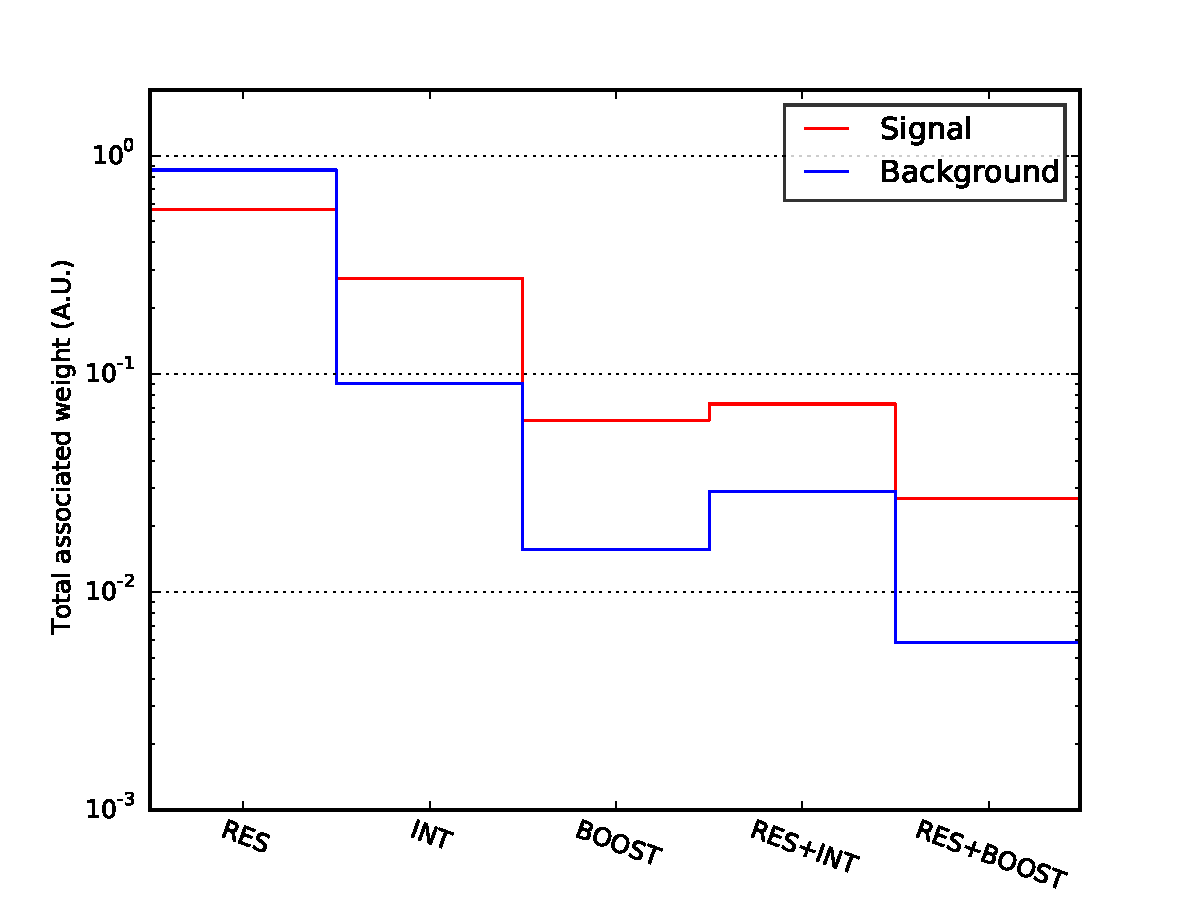
\includegraphics[width=0.65\textwidth]{plots/overlap_categories_C1.pdf}
\caption{\small The fraction of events that satisfy the requirements
  of one or more categories, for signal and background events.
}
\label{fig:categorisationHisto}
\end{center}
\end{figure}
%%%%%%%%%%%%%%%%%%%%%%%

bin 0: resolved only
bin 1: intermediate only
bin 2: boosted only
bin 3: resolved-intermediate overlap
bin 4: resolved-boosted overlap
bin 5: intermediate-boosted overlap (should be empty due to orthogonal jet multiplicity cuts) 
